\documentclass[xetex,mathserif,serif]{beamer}
\usepackage{polyglossia}
\setdefaultlanguage[babelshorthands=true]{russian}
\usepackage{minted}
\usepackage{tabu}
\usepackage[11pt]{moresize}

\useoutertheme{infolines}

\usepackage{fontspec}
\setmainfont{FreeSans}
\newfontfamily{\russianfonttt}{FreeSans}

\usepackage{textpos}
\setlength{\TPHorizModule}{1cm}
\setlength{\TPVertModule}{1cm}

\definecolor{links}{HTML}{2A1B81}
\hypersetup{colorlinks,linkcolor=,urlcolor=links}

\tabulinesep=0.7mm

\title{Архитектурные аспекты сетевой безопасности}
\subtitle{Часть 1: вопросы аутентификации}
\author[Юрий Литвинов]{Юрий Литвинов \newline \textcolor{gray}{\small\texttt{yurii.litvinov@gmail.com}}}

\newcommand{\attribution}[1] {
\vspace{-5mm}\begin{flushright}\begin{scriptsize}\textcolor{gray}{\textcopyright\, #1}\end{scriptsize}\end{flushright}
}

\date{13.05.2020г}

\begin{document}

    \frame{\titlepage}

    \section{Введение}

    \begin{frame}
        \frametitle{Сетевая безопасность}
        \begin{itemize}
            \item Почти все сервисы требуют авторизации и обеспечения безопасности
            \item Аутентификация --- установление личности (точнее, идентичности) участника взаимодействия
            \begin{itemize}
                \item Обычно взаимна
            \end{itemize}
            \item Авторизация --- установление прав на выполнение операции
            \item Шифрование --- обеспечение конфиденциальности передаваемой информации
            \item Также важны:
            \begin{itemize}
                \item Целостность --- злоумышленник ничего не поменял
                \item Актуальность --- злоумышленник не проиграл старое сообщение
            \end{itemize} 
        \end{itemize}
    \end{frame}

    \begin{frame}
        \frametitle{Некоторые соображения}
        \begin{itemize}
            \item Основные уязвимости в современных системах не технические по характеру
            \item Большинство попыток взлома --- изнутри организации
            \item Сетевая безопасность --- игра против живого, умного и часто хорошо оснащённого противника
            \begin{itemize}
                \item Задача средств безопасности --- не сделать взлом невозможным, а сделать его нерентабельным
            \end{itemize}
            \item За протоколами безопасности стоит большая наука
            \begin{itemize}
                \item Придумать свой хитрый шифр или протокол аутентификации в общем случае очень плохая идея
            \end{itemize} 
            \item tradeoff между безопасностью и удобством использования
        \end{itemize}
    \end{frame}

    \begin{frame}
        \frametitle{Шифрование}
        \begin{center}
            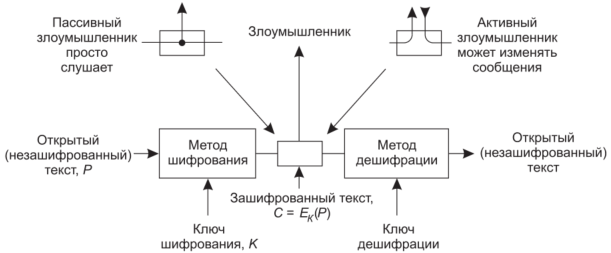
\includegraphics[width=0.6\textwidth]{cryptography.png}
            \attribution{Э. Таненбаум}
        \end{center}
        \begin{itemize}
            \item Алгоритм шифрования считается известным, секретен только ключ
            \item Усложнение алгоритма шифрования не всегда повышает криптостойкость
        \end{itemize}
        \begin{textblock}{2}(0,-6)
            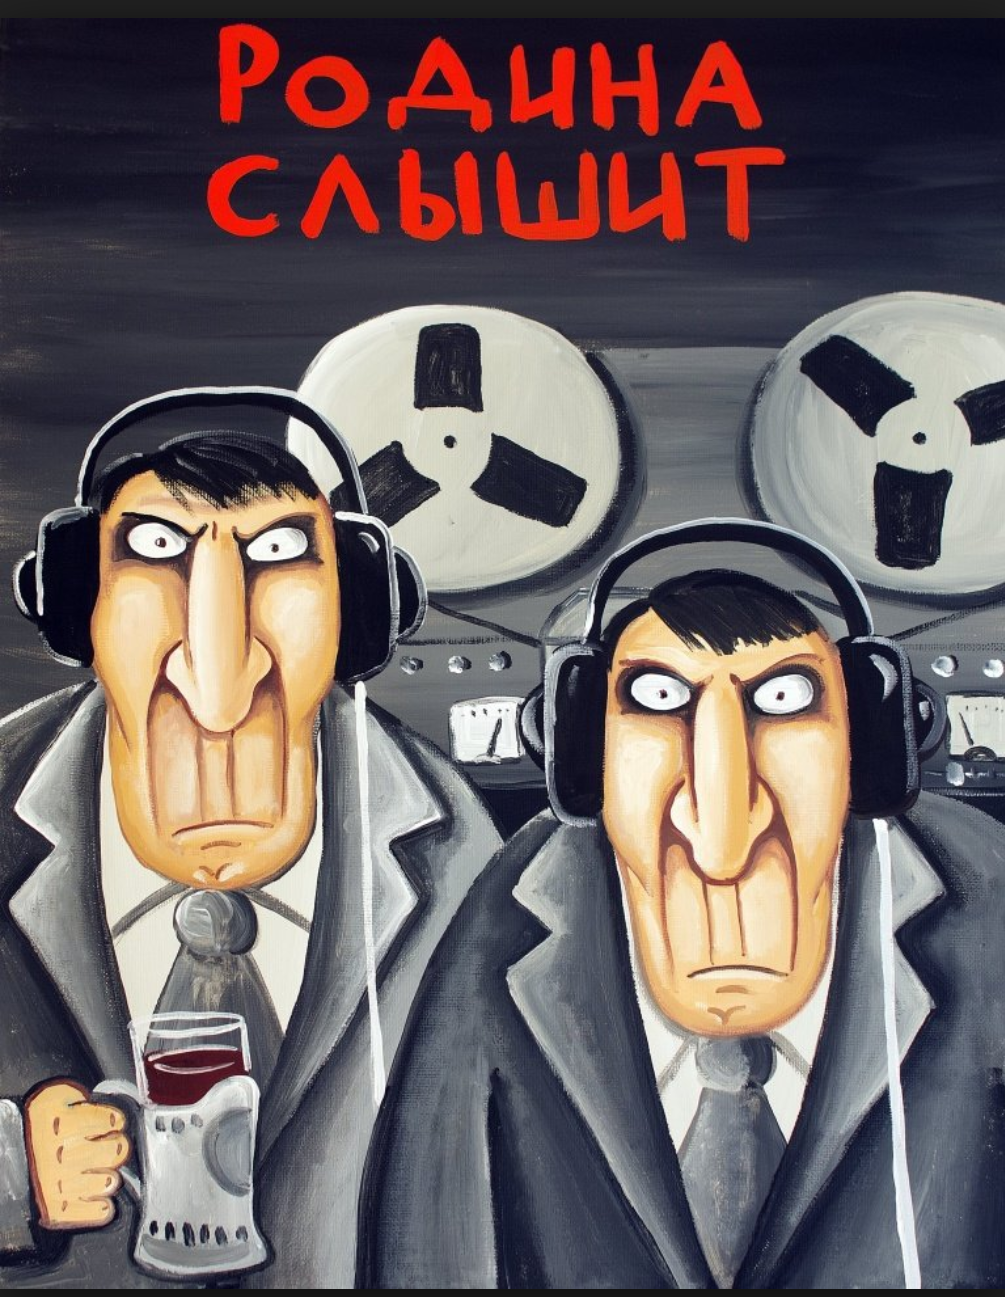
\includegraphics[width=\textwidth]{youAreBeingWatched.png}
        \end{textblock}
    \end{frame}

    \section{Сертификаты}

    \begin{frame}
        \frametitle{Предварительные знания}
        \begin{itemize}
            \item Шифрование с открытым ключом
            \begin{itemize}
                \item D и E такие что D(E(P)) = P
                \item D очень сложно получить по E
                \item E выкладывается в открытый доступ, сообщение шифруется E(P)
                \item Можно расшифровать, посчитав D(E(P)), но D хранится в тайне
            \end{itemize}
            \item Цифровая подпись
            \begin{itemize}
                \item Получатель может установить личность отправителя
                \item Отправитель не может отрицать, что он подписал сообщение
                \item Получатель не может сам подделать сообщение и сделать вид, что его послал отправитель
            \end{itemize}
        \end{itemize}
    \end{frame}

    \begin{frame}
        \frametitle{Сертификаты}
        \begin{center}
            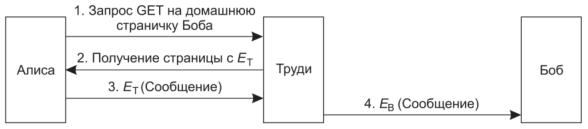
\includegraphics[width=0.6\textwidth]{manInTheMiddle.png}
            \attribution{Э. Таненбаум}
        \end{center}
        \begin{itemize}
            \item Сертификат --- сообщение, подтверждающее идентичность ключа, подписанное Certificate Authority (стандарт X.509)
            \item Цепочка сертификатов --- CA верхнего уровня подписывает сертификаты CA уровнем ниже, чтобы они могли подписывать сертификаты пользователей
            \item Корневые сертификаты --- сертификаты, которым принято доверять
            \item Самоподписанные сертификаты --- не доверенные, используются для отладки
        \end{itemize}
    \end{frame}

    \begin{frame}
        \frametitle{Применения сертификатов}
        \begin{itemize}
            \item Протокол HTTPS, проверка идентичности сервера
            \item Подписывание кода (Windows SmartScreen, Apple Code Signing)
            \item Подписывание сборок, сильные имена сборок в .NET
        \end{itemize}
        \begin{center}
            \includegraphics[width=0.6\textwidth]{dotNetCodeSigning.png}
            \attribution{J. Richter}
        \end{center}
    \end{frame}

    \begin{frame}
        \frametitle{Сертификаты (2)}
        \begin{center}
            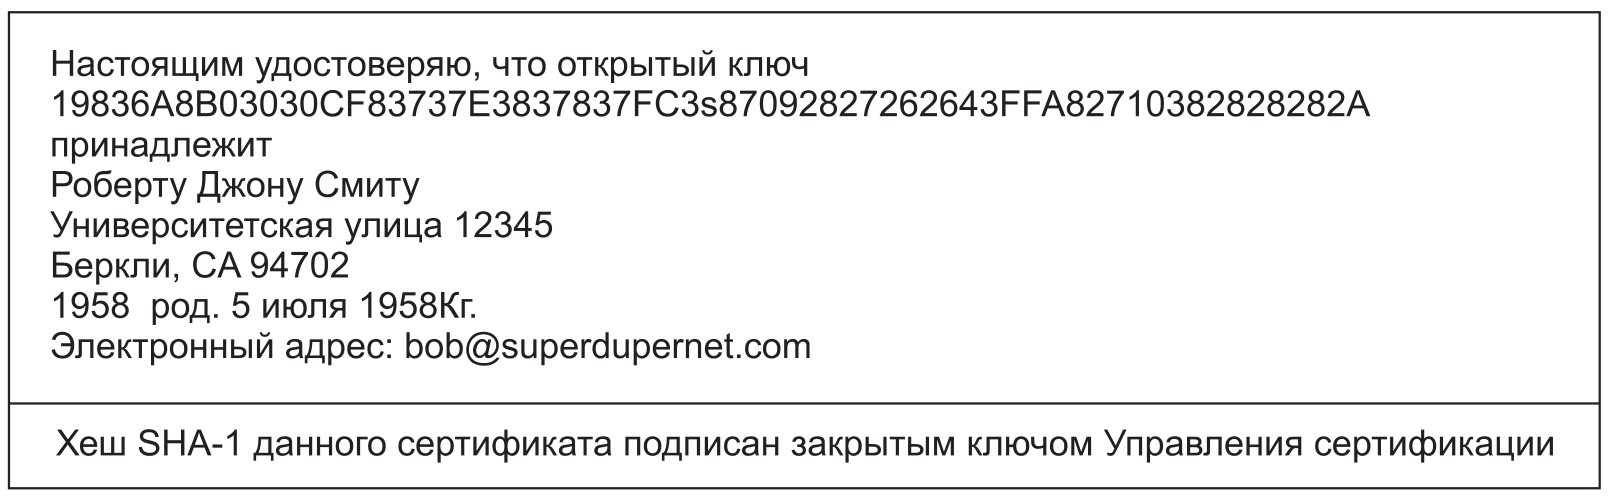
\includegraphics[width=0.75\textwidth]{certificate.png}
            \attribution{Э. Таненбаум}
        \end{center}
        \begin{itemize}
            \item Подписанный у CA сертификат стоит денег (от \$7 до более \$200 в год, в зависимости от типа)
            \begin{itemize}
                \item И требует идентификации личности (по паспорту или чему-то такому)
            \end{itemize}
            \item Сертификаты всегда выдаются на фиксированное время
            \item Сертификат можно отозвать
            \item Куча несовместимых форматов: .pem, .p12, .pfx, .der, .cer, .crt
        \end{itemize}
    \end{frame}

    \begin{frame}
        \frametitle{Certificate Authority}
        \begin{center}
            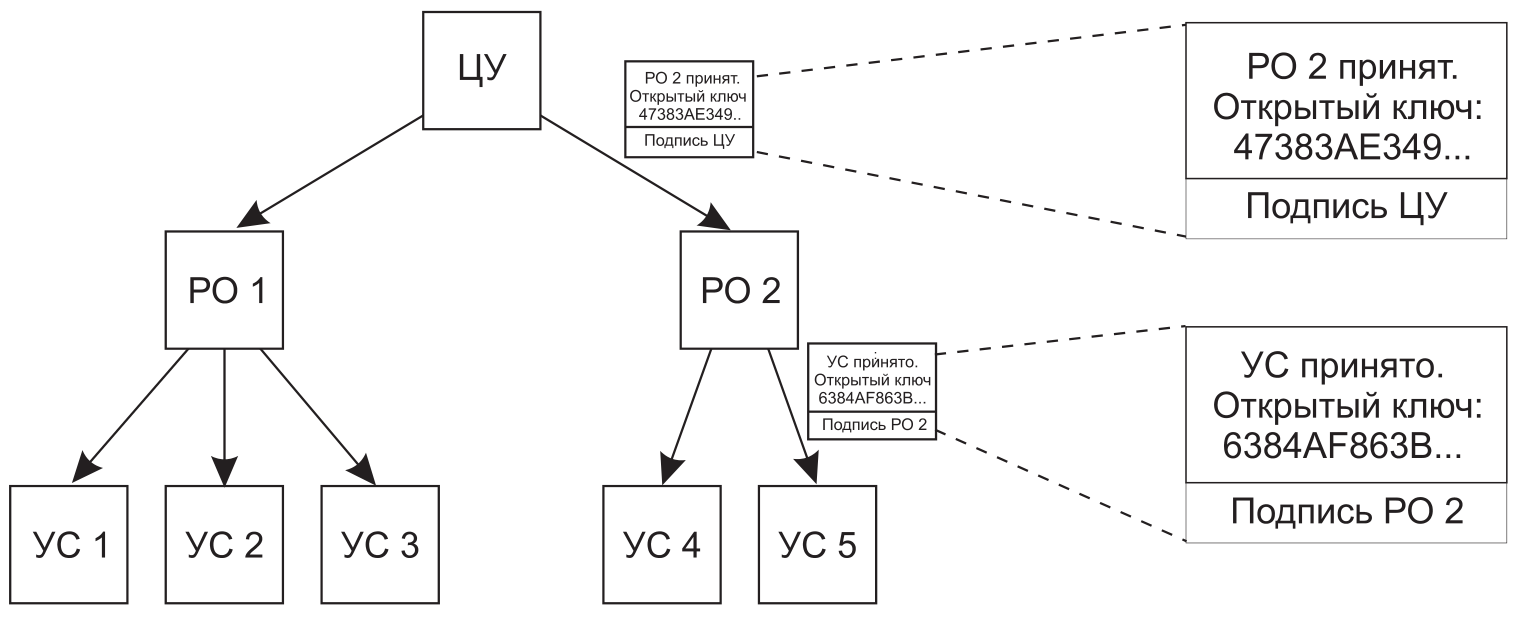
\includegraphics[width=0.85\textwidth]{certHierarchy.png}
            \attribution{Э. Таненбаум}
        \end{center}
        \begin{itemize}
            \item \url{https://letsencrypt.org/} --- автоматически и бесплатно даёт сертификаты, но им почти никто не доверяет
        \end{itemize}
    \end{frame}

    \begin{frame}
        \frametitle{Менеджер сертификатов, Windows}
        \framesubtitle{Snap-In в MMC}
        \begin{center}
            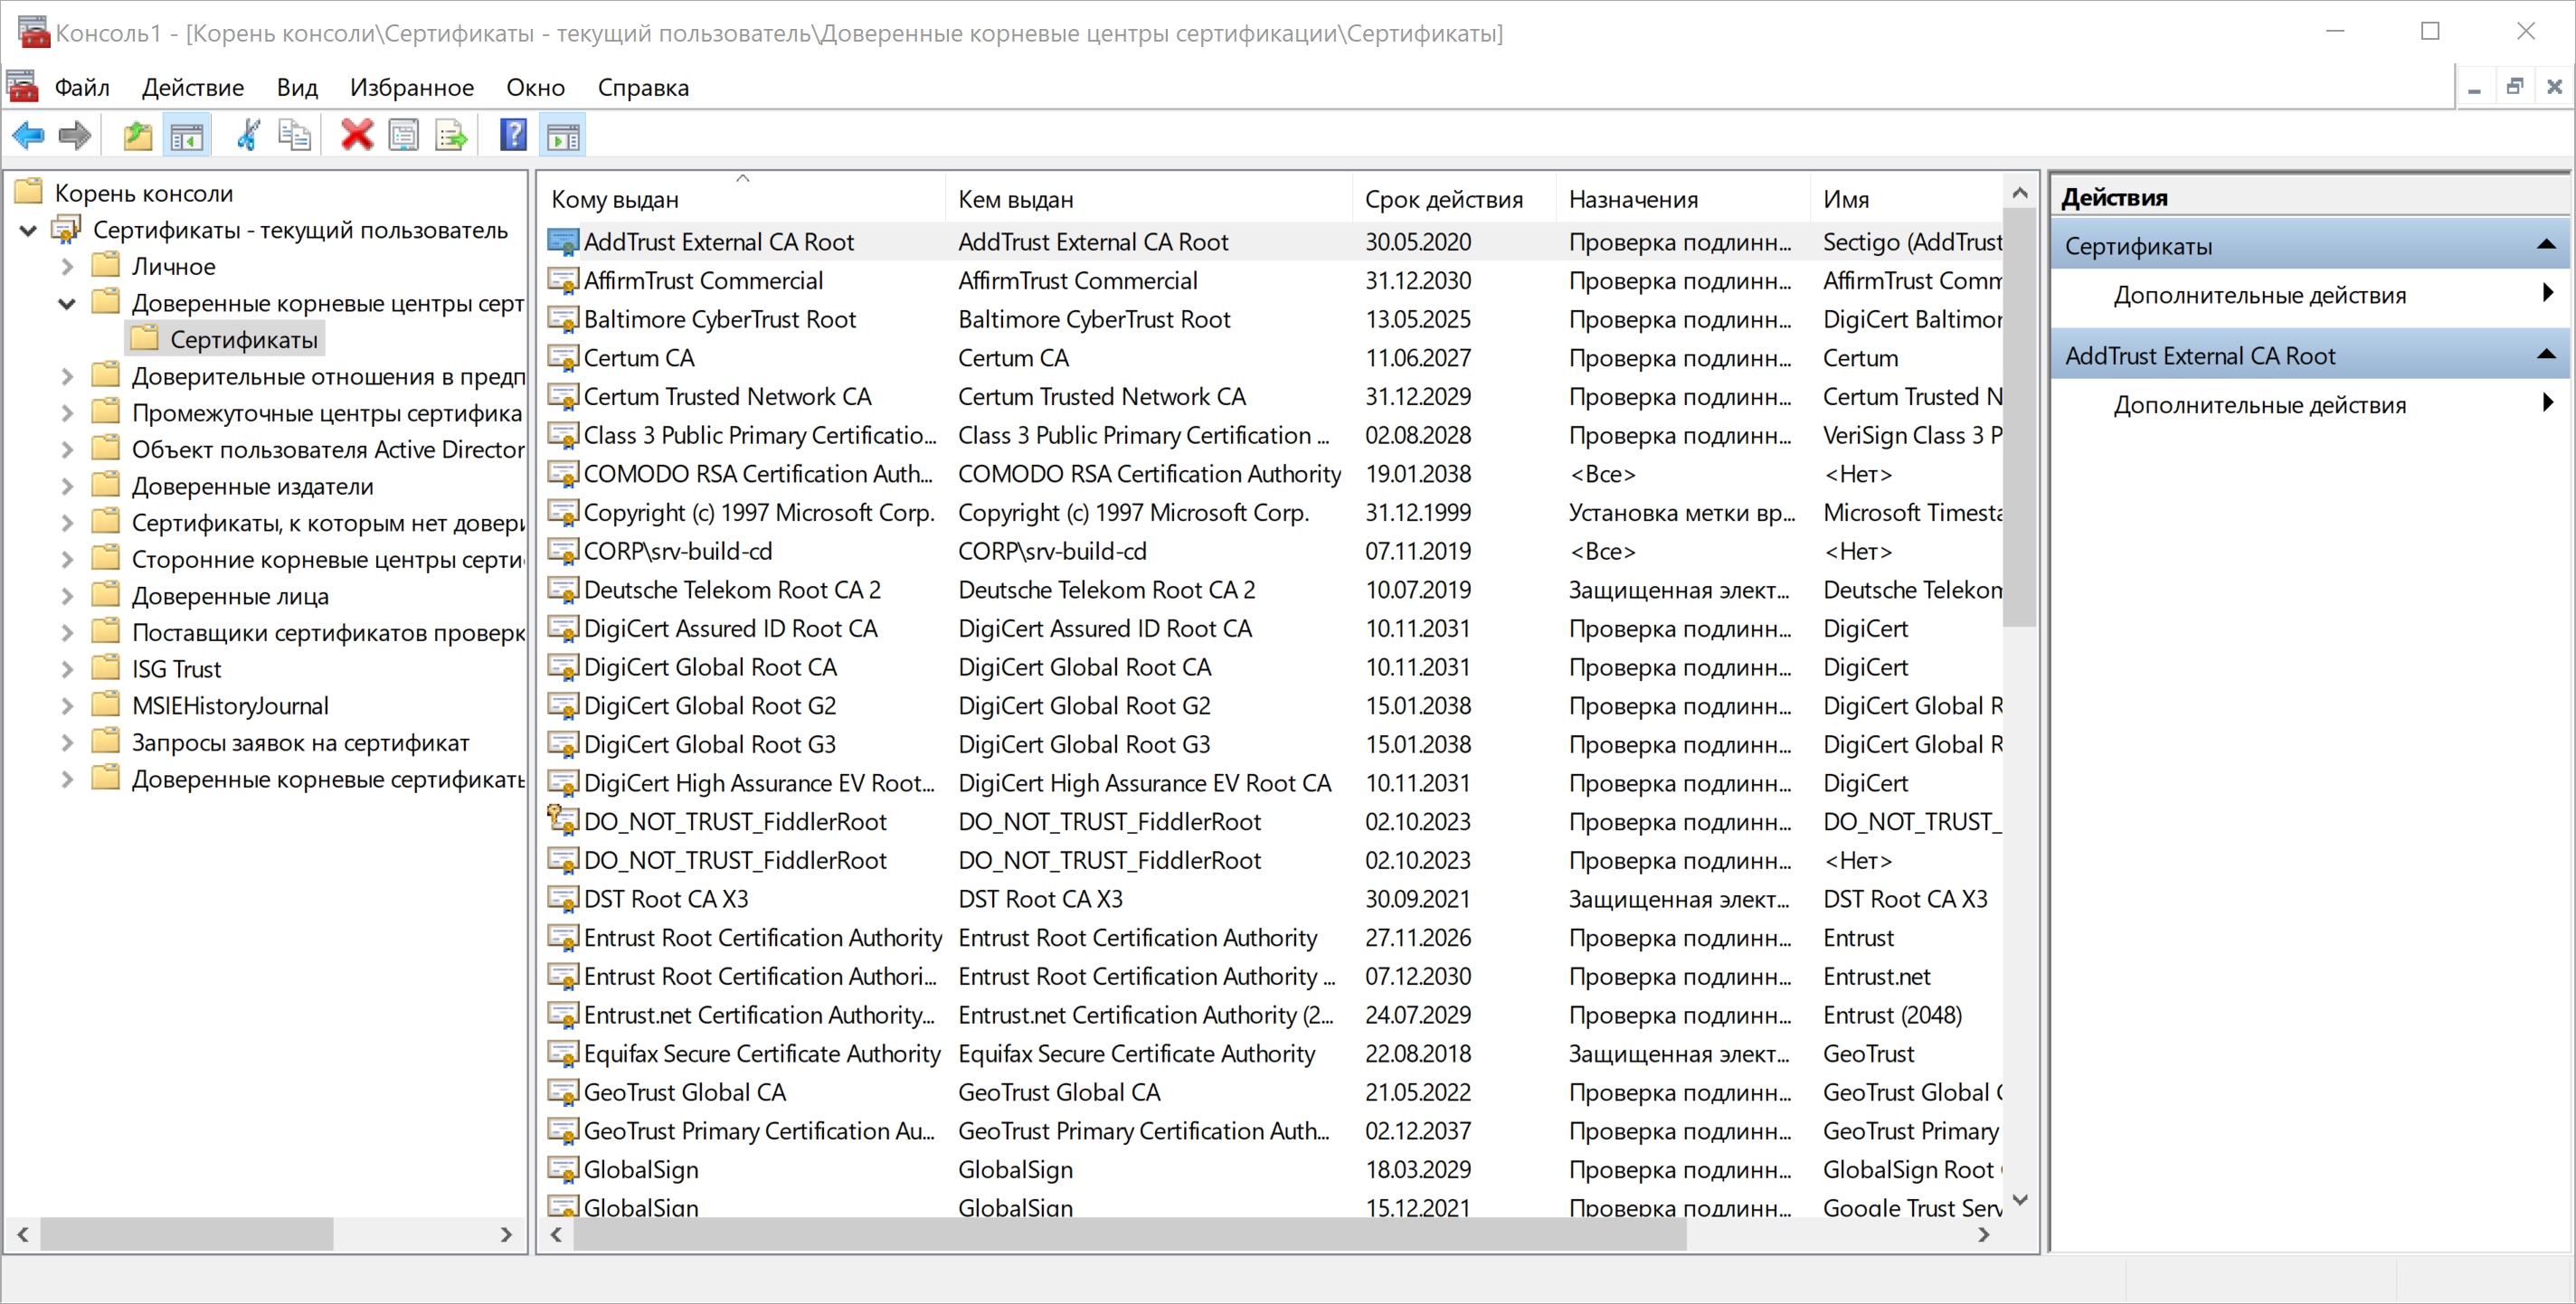
\includegraphics[width=0.95\textwidth]{windowsCertManager.png}
        \end{center}
    \end{frame}

    \begin{frame}[fragile]
        \frametitle{OpenSSL}
        \begin{itemize}
            \item OpenSSL --- библиотека и набор инструментов для криптографии и работы с протоколами SSL/TLS
            \item Стандарт де-факто для работы с открытыми ключами, сертификатами и т.д.
            \item Как сгенерить самоподписанный сертификат:
            
                \begin{minted}{bash}
openssl req -x509 -nodes -days 365 
    -newkey rsa:2048 -keyout privatekey.key 
    -out certificate.crt
                \end{minted}
        \end{itemize}
    \end{frame}

    \section{Аутентификация}

    \subsection{Общий ключ}

    \begin{frame}
        \frametitle{Аутентификация Challenge-Response с общим ключом}
        \begin{center}
            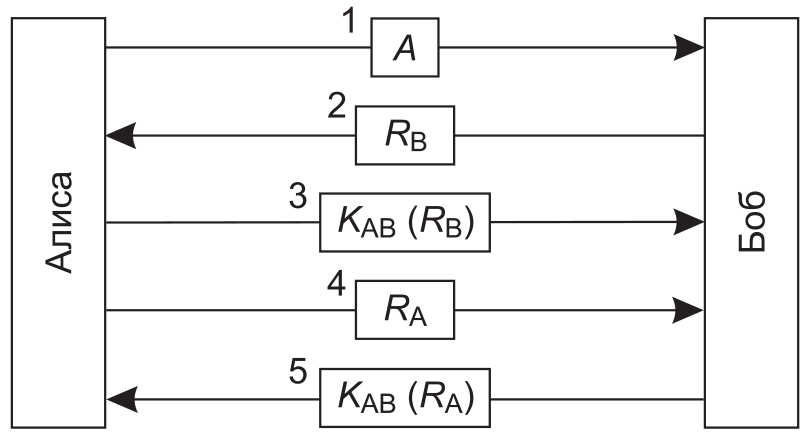
\includegraphics[width=0.5\textwidth]{challengeResponse.png}
            \attribution{Э. Таненбаум}
        \end{center}
        \begin{itemize}
            \item $R_B$ --- \textbf{nonce} (number used once), для предотвращения атаки повтором
            \item $K_{AB}$ --- общий ключ
        \end{itemize}
    \end{frame}

    \begin{frame}
        \frametitle{``Упрощённый'' протокол}
        \begin{center}
            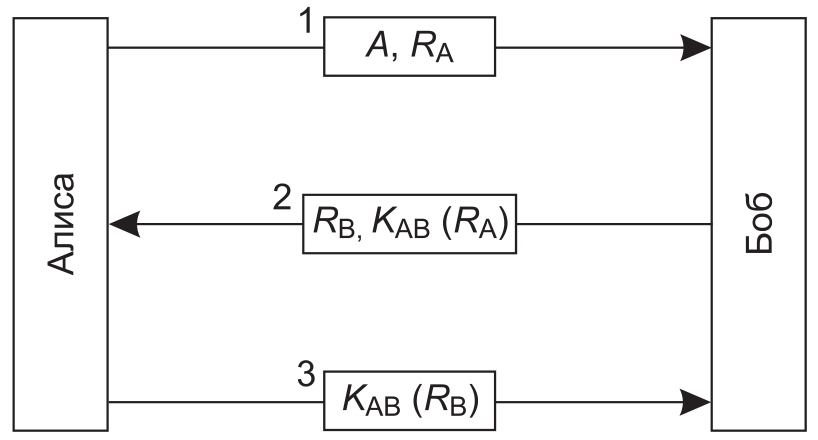
\includegraphics[width=0.5\textwidth]{simpleChallengeResponse.png}
            \attribution{Э. Таненбаум}
        \end{center}
    \end{frame}

    \begin{frame}
        \frametitle{Зеркальная атака}
        \begin{center}
            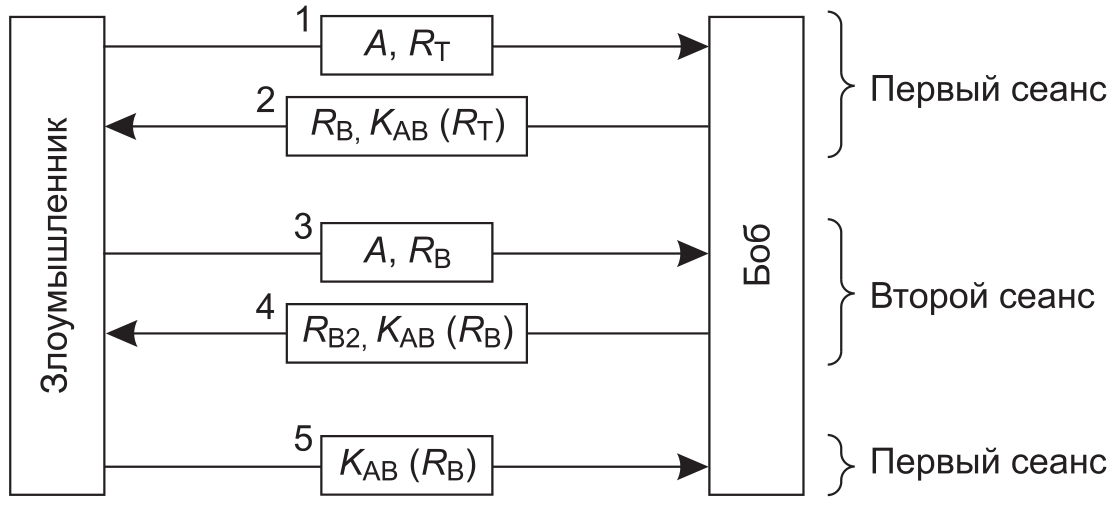
\includegraphics[width=0.65\textwidth]{mirrorAttack.png}
            \attribution{Э. Таненбаум}
        \end{center}
        \vspace{5mm}
        \textbf{Разработать корректный протокол аутентификации сложнее, чем это может показаться}
    \end{frame}

    \begin{frame}
        \frametitle{Правильный протокол}
        \begin{center}
            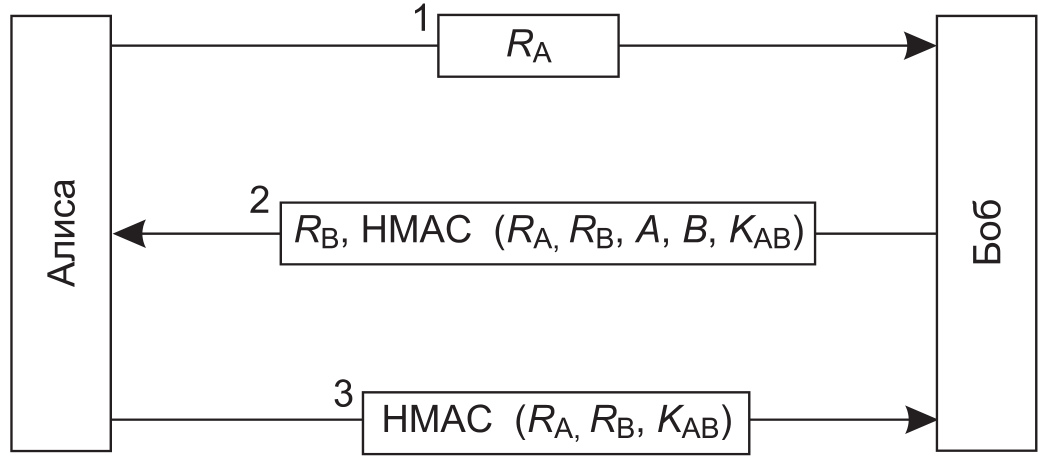
\includegraphics[width=0.6\textwidth]{hmacs.png}
            \attribution{Э. Таненбаум}
        \end{center}
        \begin{itemize}
            \item HMAC --- Hashed Message Authentication Code
        \end{itemize}
    \end{frame}

    \begin{frame}
        \frametitle{Как на самом деле}
        \begin{itemize}
            \item Basic Authentication --- логин и пароль передаются нешифрованными в заголовке HTTP-запроса
            \item HTTPS обеспечивает безопасность
            \item Сервер возвращает Access Token
            \item Access Token предъявляется при каждом следующем запросе
            \begin{itemize}
                \item Имеет ограниченное время жизни, но его можно продлять
            \end{itemize}
            \item Пароли не хранятся на сервере, хранятся их хеши
            \begin{itemize}
                \item Salt --- случайное число, дописываемое к паролю на стороне сервера, хранится вместе с хешем пароля
                \item Если базу паролей украдут, узнать исходные пароли очень сложно
            \end{itemize}
        \end{itemize}
    \end{frame}

    \subsection{Открытый ключ}

    \begin{frame}
        \frametitle{Алгоритм Диффи-Хеллмана}
        \begin{center}
            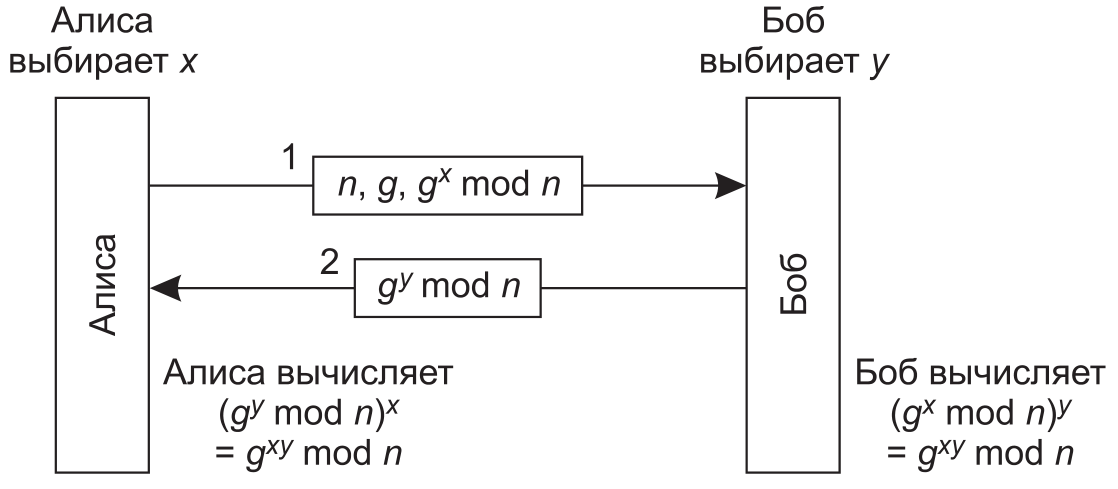
\includegraphics[width=0.6\textwidth]{diffieHellman.png}
            \attribution{Э. Таненбаум}
        \end{center}
    \end{frame}

    \begin{frame}
        \frametitle{Атака ``Man In The Middle''}
        \begin{center}
            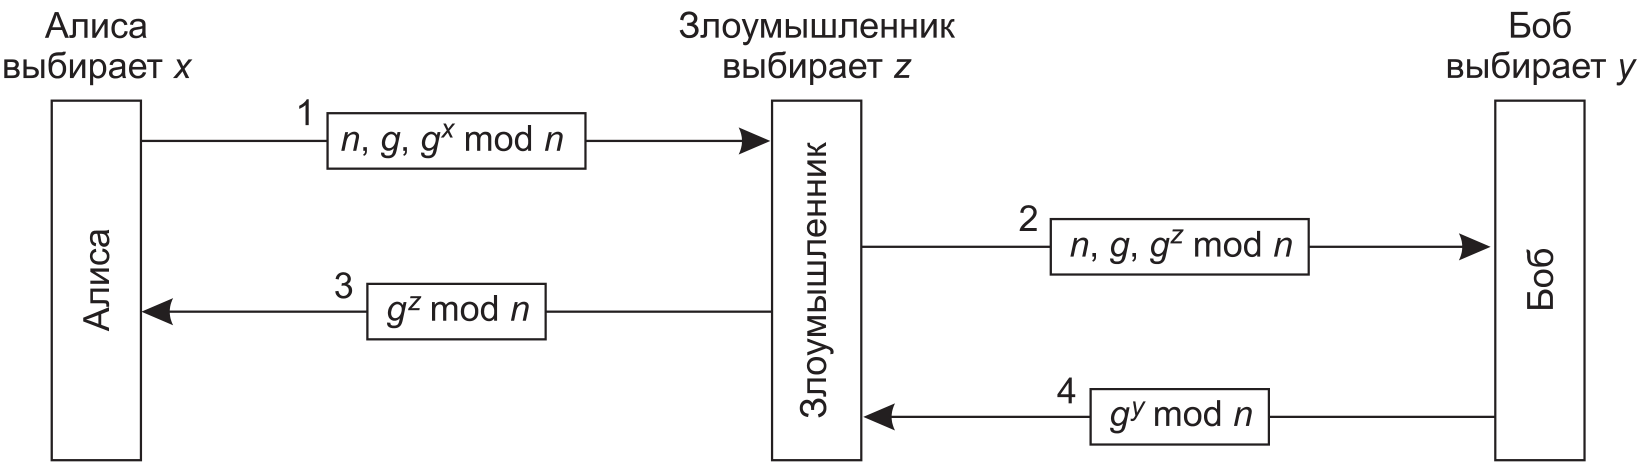
\includegraphics[width=0.9\textwidth]{diffieHellmanMitm.png}
            \attribution{Э. Таненбаум}
        \end{center}
    \end{frame}

    \begin{frame}
        \frametitle{Аутентификация с открытым ключом}
        \begin{center}
            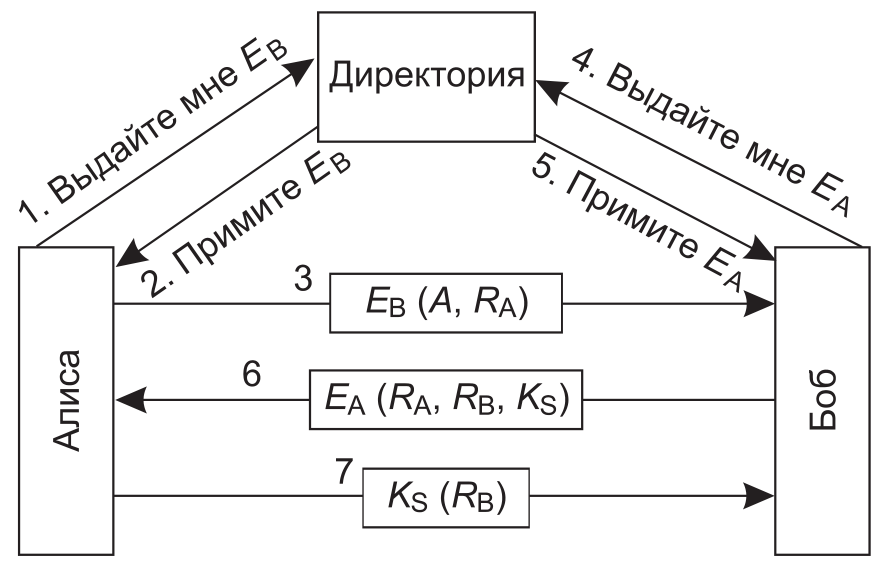
\includegraphics[width=0.6\textwidth]{openKeyAuthentication.png}
            \attribution{Э. Таненбаум}
        \end{center}
        \begin{itemize}
            \item $E_A$, $E_B$ --- открытые ключи Алисы и Боба
            \item $R_A$, $R_B$ --- nonce
        \end{itemize}
    \end{frame}

    \section{Безопасность транспортного уровня}

    \begin{frame}
        \frametitle{HTTPS}
        \begin{center}
            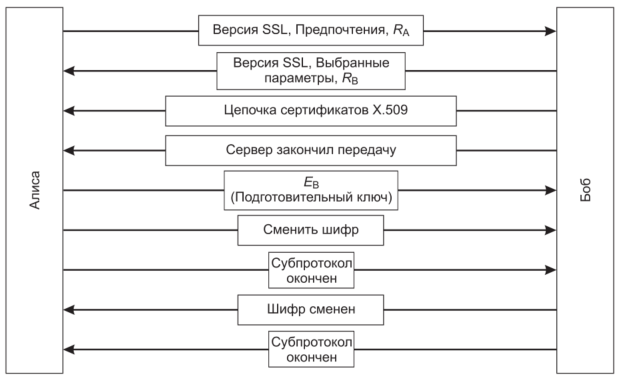
\includegraphics[width=0.6\textwidth]{ssl.png}
            \attribution{Э. Таненбаум}
        \end{center}
        \begin{itemize}
            \item SSL (Secure Sockets Layer)
            \item HTTPS --- HTTP через SSL
            \item Порт 443
            \item Аутентифицируется только сервер
        \end{itemize}
    \end{frame}

    \begin{frame}
        \frametitle{SSL, транспортный субпротокол}
        \begin{center}
            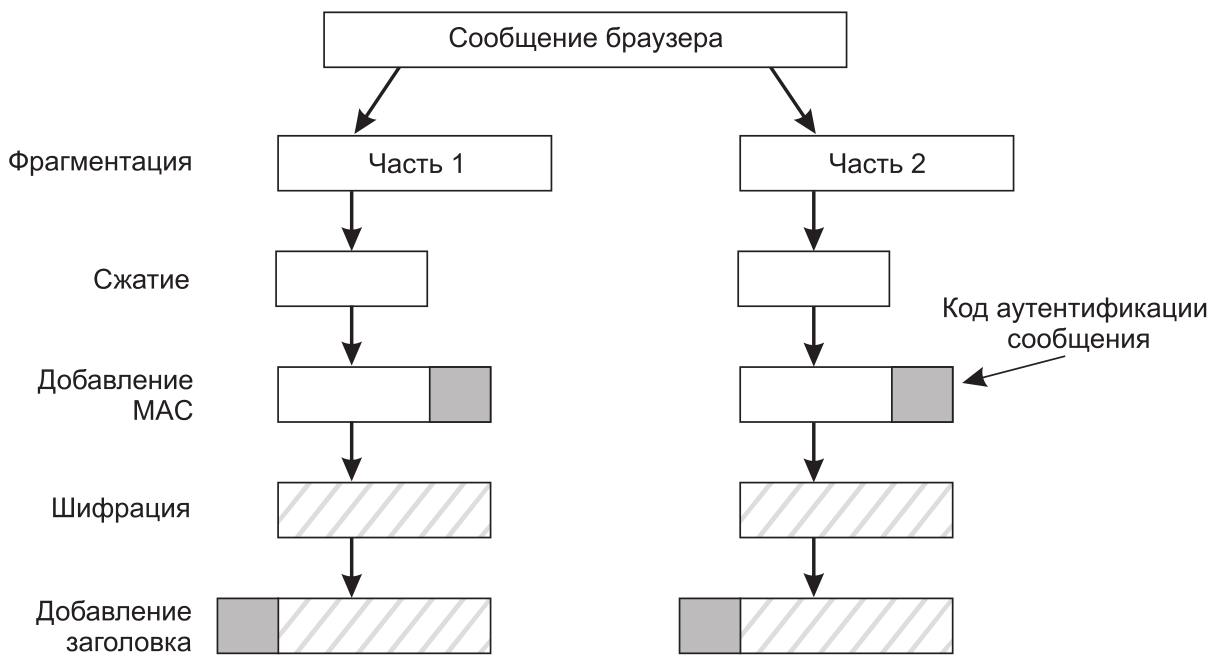
\includegraphics[width=0.6\textwidth]{sslCommunication.png}
            \attribution{Э. Таненбаум}
        \end{center}
        \begin{itemize}
            \item Triple DES + SHA-1
            \item Или RC4 со 128-битным ключом + MD5
            \item TLS --- Transport Layer Security (продвинутый SSL)
        \end{itemize}
    \end{frame}

    \begin{frame}
        \frametitle{DNS Spoofing}
        \begin{columns}
            \begin{column}{0.4\textwidth}
                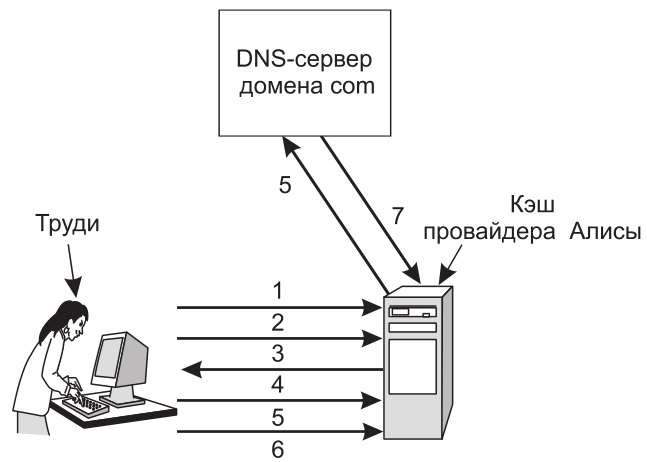
\includegraphics[width=0.95\textwidth]{dnsSpoofing.png}
                \attribution{Э. Таненбаум}
            \end{column}
            \begin{column}{0.6\textwidth}
                \begin{footnotesize}
                    \begin{enumerate}
                        \item Запрос foobar.trudy-the-intruder.com (чтобы trudy-the-intruder.com попал в кеш провайдера)
                        \item Запрос www.trudy-the-intruder.com (чтобы получить следующий порядковый номер провайдера)
                        \item Запрос об адресе www.trudy-the-intruder.com к нашему DNS
                        \item Запрос к bob.com
                        \item Запрос о bob.com к DNS зоны com
                        \item Подделанный ответ о bob.com
                        \item Настоящий ответ, отвергнутый, потому что уже поздно
                    \end{enumerate}
                \end{footnotesize}
            \end{column}
        \end{columns}
    \end{frame}

    \begin{frame}
        \frametitle{Результат}
        \begin{center}
            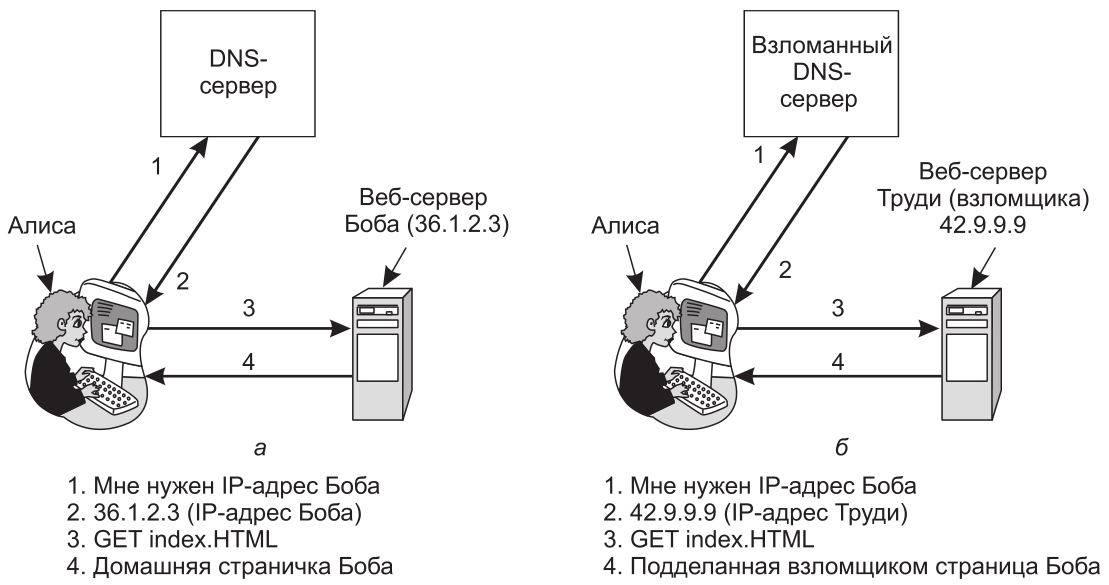
\includegraphics[width=0.9\textwidth]{dnsSpoofingResult.png}
            \attribution{Э. Таненбаум}
        \end{center}
    \end{frame}

    \section{Задача}

    \begin{frame}
        \frametitle{Задача на остаток пары}
        \begin{footnotesize}
            Прикрутить аутентификацию по X.509-сертификатам к чатам на RabbitMQ с прошлой практики
            \begin{itemize}
                \item Подробная инструкция: \url{https://www.rabbitmq.com/ssl.html}
                \item Аутентификация обоюдная: сервер проверяет клиент, клиент проверяет сервер
                \item Обратите внимание:
                \begin{itemize}
                    \item У JVM своя (довольно удобная вроде) подсистема работы с сертификатами, у .NET тоже
                    \item Может быть полезно \url{https://www.rabbitmq.com/troubleshooting-ssl.html}
                    \item В общем случае генерим самоподписанный CA-сертификат и генерим с его помощью сертификат сервера
                    \item Можно и клиента (или отдельный CA для клиента, но сервер должен ему доверять)
                    \item См. \url{https://www.rabbitmq.com/ssl.html\#peer-verification-trusted-certificates}
                \end{itemize}
                \item За 15 минут до конца пары собираемся и показываем результаты
            \end{itemize}
        \end{footnotesize}
    \end{frame}

\end{document}